\newif\ifdebug
%\debugtrue
\ifdebug
\documentclass[12pt,a4paper]{ctexrep}
\usepackage[a4paper, portrait, margin=0.8in]{geometry}
\usepackage{graphicx} % Required for inserting images
\usepackage{amsmath}
\usepackage{amsfonts}
\usepackage{amssymb}
\usepackage{amsthm}
\usepackage{markdown}
%\usepackage{china2e} 
\usepackage[utf8]{inputenc}
\usepackage[colorlinks,linkcolor=blue]{hyperref}
\begin{document}
\fi

\chapter{Counting计数, 组合}
Counting, Permutations, Combinations, Balls and Walls, Principle of Inclusion and Exclusion, Generalized Principle of Inclusion and Exclusion, Pigeonhole Principle
\section{定义}
\subsection{Definition of 名词}
Permutations: 排列. [n] = $\{1,2,\dots,n\}$\\$\indent$
Onto:单射.\\$\indent$
\section{定理/结论}
\subsection{几何意义}
[n] has $2^{n}$ subsets\\$\indent$
$\binom{n}{0} + \binom{n}{1} + \binom{n}{2} + \dots + \binom{n}{n} = 2^{n}$\\$\indent$
$\sum_{i=0}^{n} (-1)^{n} \binom{n}{i} = 0$ $\Leftarrow$ even sized subsets=odd sized subsets\\$\indent$
$n \binom{n-1}{k} = (k+1) \binom{n}{k+1}$ $\Leftarrow$ want to choose k+1 people from n people and designate a captain\\$\indent$
$\star \binom{n}{r} = \binom{n-1}{r}+\binom{n-1}{r-1}$ $\Leftarrow$ number of subsets with an arbitrary element + without the element\\$\indent$
$\sum_{0\leq j\leq i\leq n} \binom{n}{i}\binom{i}{j} = 3^{n}$ $\Leftarrow$ separate n into 3 parts\\$\indent$
$\binom{n}{r} = \binom{n}{n-r}$
\subsection{结论}
for [n], how many permutations $\pi$ have the property $\forall i, \pi[i] \neq i$ : $d_{n} = (d_{n-1}+d_{n-2})(n-1)$
\subsection{PIE}
Principle of inclusion and exclusion(PIE): Find the whole number of elements in $A_{1} \sim A_{n}$. \\$\indent$
Generalized PIE: Find the number of elements $E(m)$ appearing in exactly $m$ of $A_{1} \sim A_{n}$. \\$\indent$
$\star$经典习题:6 persons, every pair is either friends or enemy.$\Rightarrow$There must exist 3 people who are friends to each other or enemies to each other.
\section{重要定理详解}
\subsection{PIE}
Let $A_{1}, A_{2}, \dots , A_{n}$ be finite sets.

Suppose $x$ is in exactly $r$ of the $n$ sets.

This indicates that $x$ is counted in $\binom{r}{1} \, A_{n}$ s, $\binom{r}{2} \, A_{n_{1}}\cap A_{n_{2}}$ s,$\dots$, $\binom{r}{r} \, A_{n_{1}}\cap A_{n_{2}} \cap \dots \cap A_{n_{r}}$ s.

$\because$ $-\binom{r}{0}+\binom{r}{1}-\binom{r}{2}+\dots+(-1)^{r+1}\binom{r}{r} +\binom{r}{0}= $ number of subsets with odd sizes - number of subsets with even sizes+1 = 1

$\therefore$Set $\omega(t) = \sum_{i_{1},i_{2},\dots,i_{t}}|A_{i_{1}} \cap A_{i_{2}} \cap \dots \cap A_{i_{t}}|$

$\therefore$ \[|\cup_{i=1}^{k} A_{i}| = \sum_{t=1}^{k} (-1)^{t+1} \omega(t)\]

重点在于找$A_{1},A_{2},\dots,A_{n}$!!!\\

\begin{center}
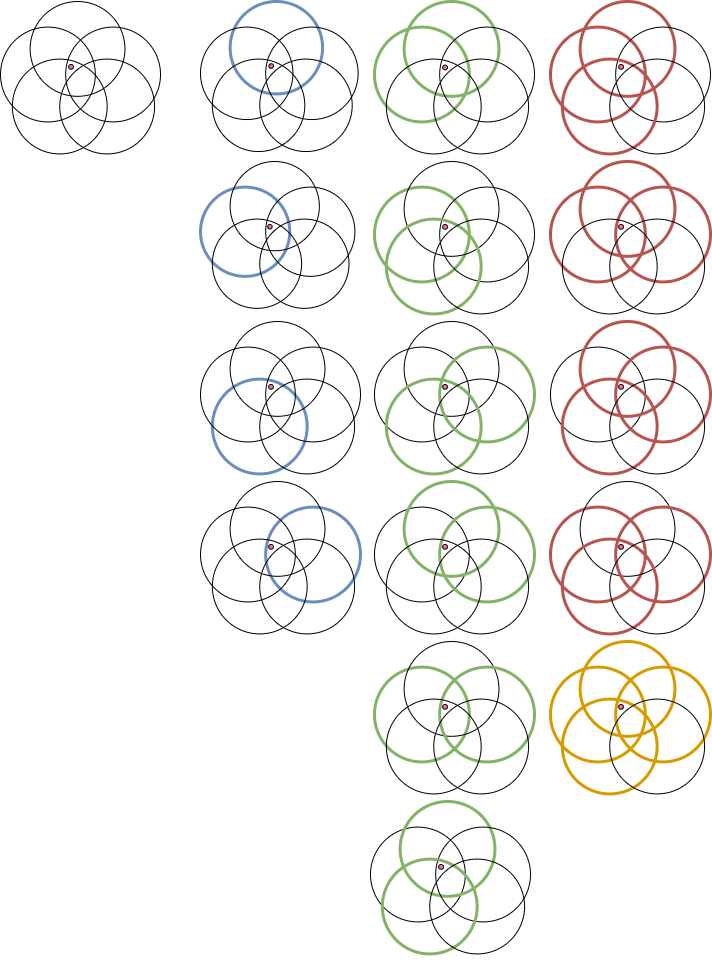
\includegraphics[scale=0.3]{PIE.png}
\end{center}

\subsection{Generalized PIE}
in a universe with n elements, $A_{1}, A_{2}, \dots , A_{n}$ are finite sets.

$\omega(t) = \sum_{i_{1},i_{2},\dots,i_{t}}|A_{i_{1}} \cap A_{i_{2}} \cap \dots \cap A_{i_{t}}|$

$E(m)$ = the number of elements appearing in exactly $m$ of $A_{1} \sim A_{n}$ = \[\sum_{k=m}^{n} (-1)^{k-m} \binom{k}{m} \omega(k)\]

An example are as follows:  \href{https://www.youtube.com/watch?v=D1T3xy_vtxU}{vid}

\begin{center}
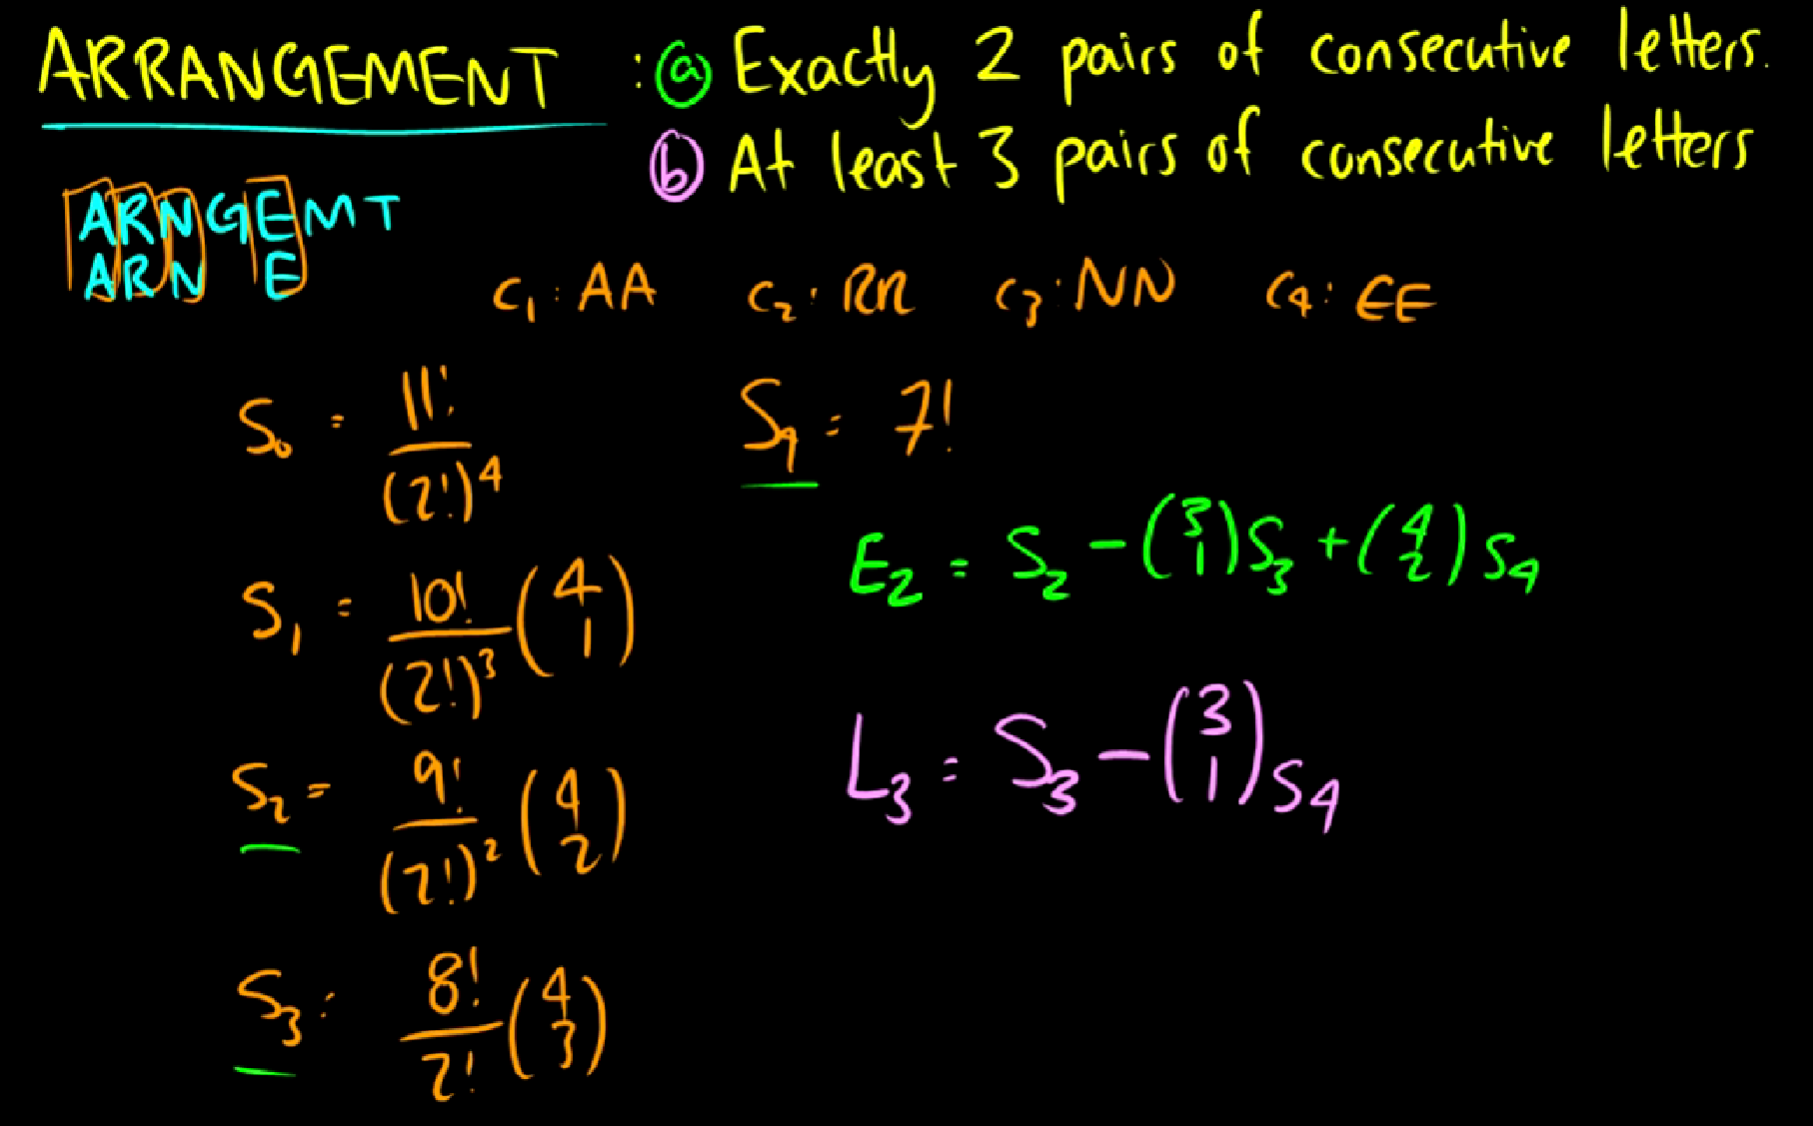
\includegraphics[scale=0.3]{PIE_Example.png}
\end{center}

\section{方法}
Principle of Addition (Case work principle)

Principle of Multiplication

算排列的时候别忘了去重

合理使用induction

插板法

$\indent\star$题目较长的时候,要么用Pigeon-Hole Principle,要么用induction/strong induction

\section{例题}
\subsection{插板法}
How many solutions do we have if $x_1+x+2+x_3+x_4 = 10, x_i \in N$: We have 10 balls and 3 walls, we have $\binom{13}{3}$ solutions.

\subsection{People sitting around circles}
How many ways can $n$ people sit around $r$ circles: 

Let $s(n,r)$ be the ways $n$ people can sit around $r$ circles. Then a person $n$ can sit in his own circle or share a circle with others, therefore $s(n,r) = s(n-1,r-1)+(n-1)s(n-1,r)$.

$\Rightarrow$ if $r=1$, $s(n,1)=(n-1)!$.

\subsection{PIE}
\subsubsection{$n$ students and none of them sit in their chair}
$d_0=1$, $d_1=0$, do induction, when adding a student, let that student sit in $i$'s position, $i$ can sit in $n$'s position, thus $d_{n-2}$, or $i$ can sit in other positions, thus $d_{n-1}$. Therefore, $d_n=d_{n-1}+d_{n-2}$

Extension: How many permutations $\pi$ of $[n]$ have exactly $k$ fixed points? : First select $k$ elements from $n$ elements, then it's a permutation of $n-k$ elements which are not in their own places. Therefore, there's $d_{n,k}=\binom{n}{k} d_{n-k}$

By PIE, let $S_i$ is the number of permutations that has $i$ fixed points, then the number of permutations where no $\pi[i]=i$ is $d_n=n! - (\sum_{i=1}^n (-1)^{n+1}\binom{n}{i} S_i) = \dots = n! \sum_{i=1}^n \frac{(-1)^{i}}{i!}$

\subsubsection{How many functions from $[n]$ to $[m]$ are onto}
Number of functions that do not cover the element $i$ in $[m]$ : $|A_i| = (m-1)^n$, then the number of functions that do not cover $k$ elements in $[m]$ are \[S_k = \binom{n}{k} |\cap_{i=a_1,a_2,\dots,a_k} A_i| = \binom{n}{k} (m-k)^n.\] The number of functions that are onto from $[n]$ to $[m]$ are \[O(n,m) = m^n-|\cup_{i=1}^m A_i| = m^n-(\sum_{i=1}^m (-1)^{i+1} S_i = m^n-(\sum_{i=1}^n (-1)^{i+1} \binom{n}{i}(m-i)^n\]

\subsection{PigeonHole Principle}
\subsubsection{choose 10 points from a 3x3 square, there must be two points whose distance < $\sqrt{2}$}
there must be a square of 1x1 where two points are in it, these two points' distance $< \sqrt{2}$
\subsubsection{$\exists x,y \in N, 2024|9^x-9^y$}
$\iff$ $9^x \equiv 9^y$ (mod 2024), because there's only 2024 kinds of remainders when divided by 2024, so when chosen 2025 numbers, there must exist two numbers that has the same remainder.
\subsubsection{There are 6 candidates for president. Every pair of candidates is either friends or enemies. Prove that there are either 3 candidates who are all friends or 3 candidates who are all enemies.}
for a candidate, there's 5 pairs of relations with him, so there must be at least 3 pairs of same relations. Set $A$ is in the same relation with $B,C,D$, if $B,C,D$ are pairwise not in the same relation as $A$, then $B,C,D$ are of the same relation, proofing the assumption. Otherwise, $A$ and the two of them are in the same relation, proofing the assumption.

\ifdebug
\end{document}
\fi